\documentclass{article}
%Preamble
\usepackage{float}
\usepackage{color}
\usepackage{listings}
\usepackage{longtable}
\usepackage{amsmath,amssymb}
\usepackage{graphics}
\usepackage{graphicx}

\title{AE 622 - Computing of high speed flows\\ Assignment 5: Report \\ Simulation of 2D scramjet intake}
\author{Vinod Kumar Metla - 130010048\\Aditi Taneja - 13D100026}
\date{\today}

\begin{document}
\pagenumbering{arabic}
\maketitle
\newpage

\section*{Introduction}
A 2D inlet for a scramjet is simulated with Mach number 5.5 and angle of attack $-3^o$ and compared with inviscid theory results as well as with design geometry (i.e. at Mach 6.5 and zero angle of attack). 3000 iterations were performed and residue was plotted.
Total Pressure ratios, Temperature ratios and overall total pressure ratios across the shocks were compared.

\section*{Plots}
\subsection*{M = 6.5, aoa = 0}
\begin{figure}[H]   \label{figure}
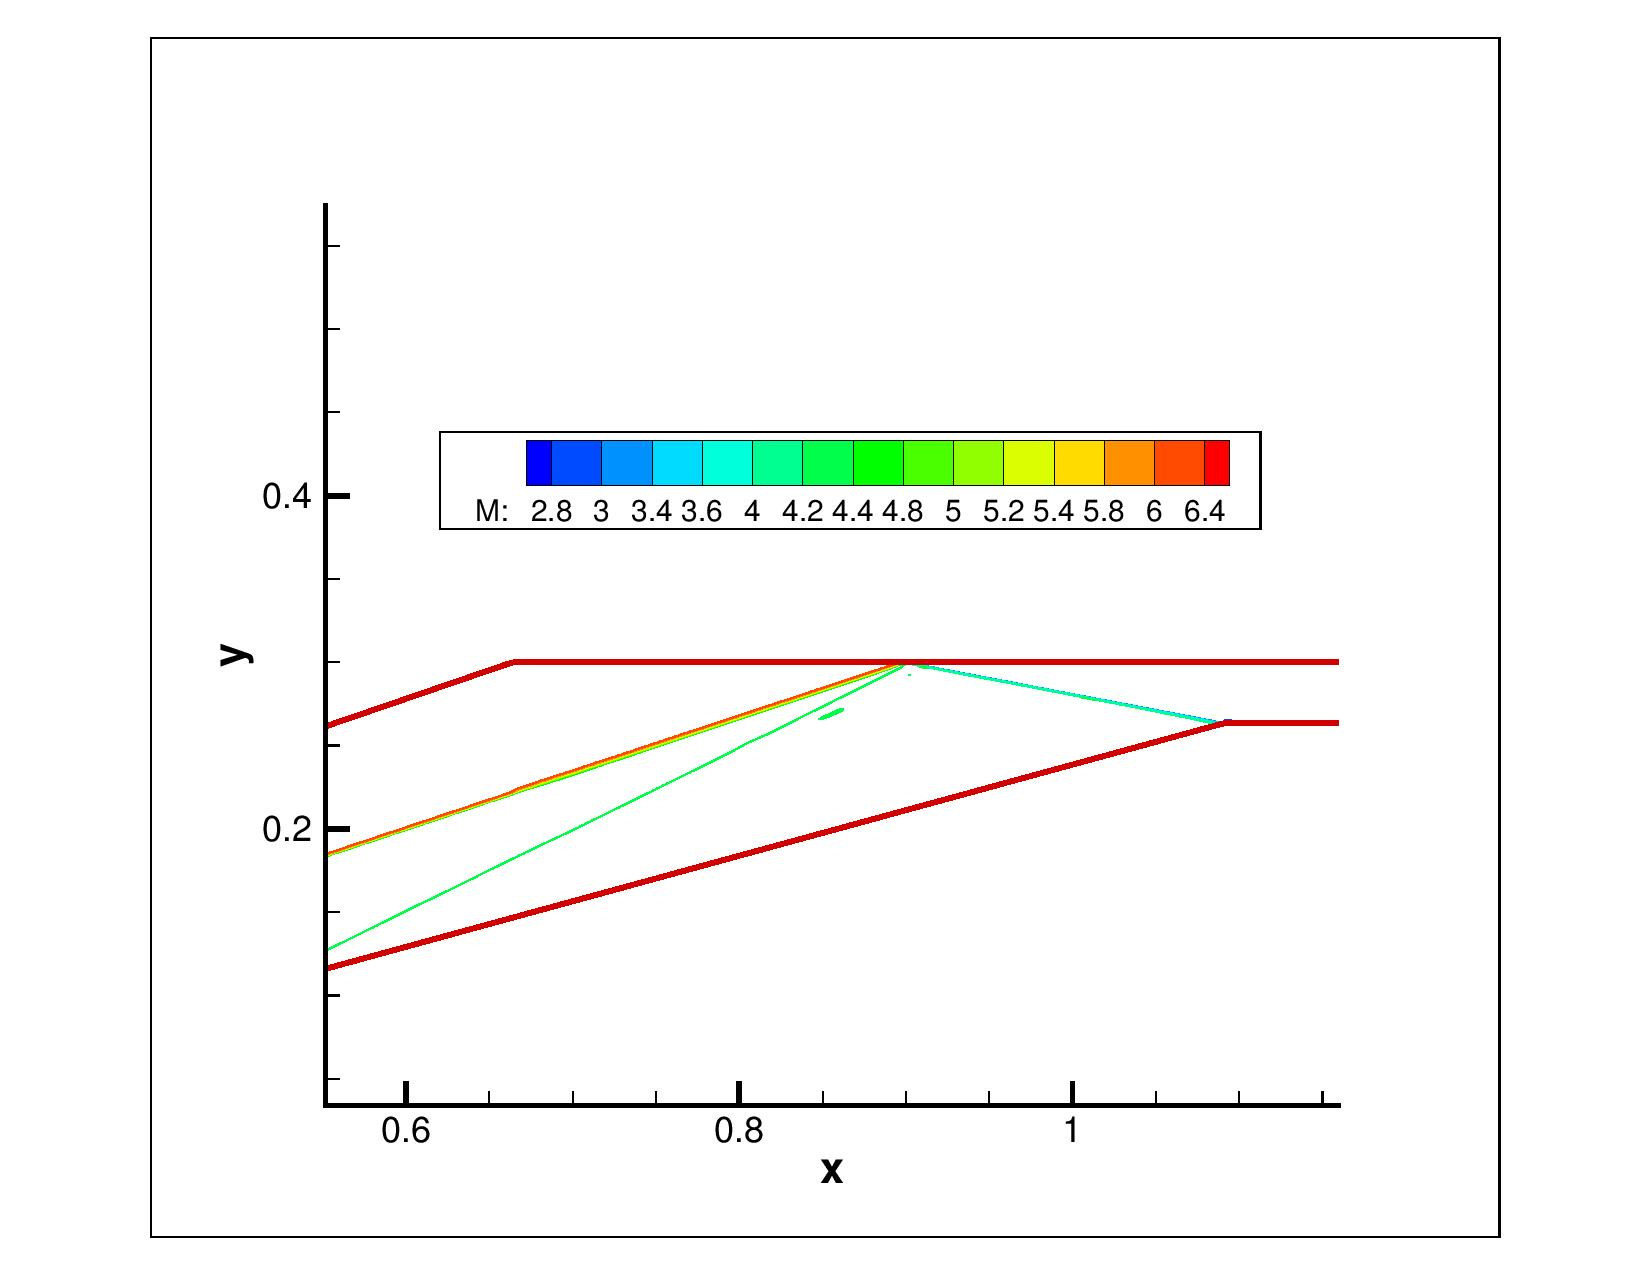
\includegraphics[width=10cm]{6.5/M_cont_1.jpg}		%%%%%%%%%%%change location and name
\label{figure:}
\caption{Mach number Contour Plot}
\end{figure}

\begin{figure}[H]   \label{figure}
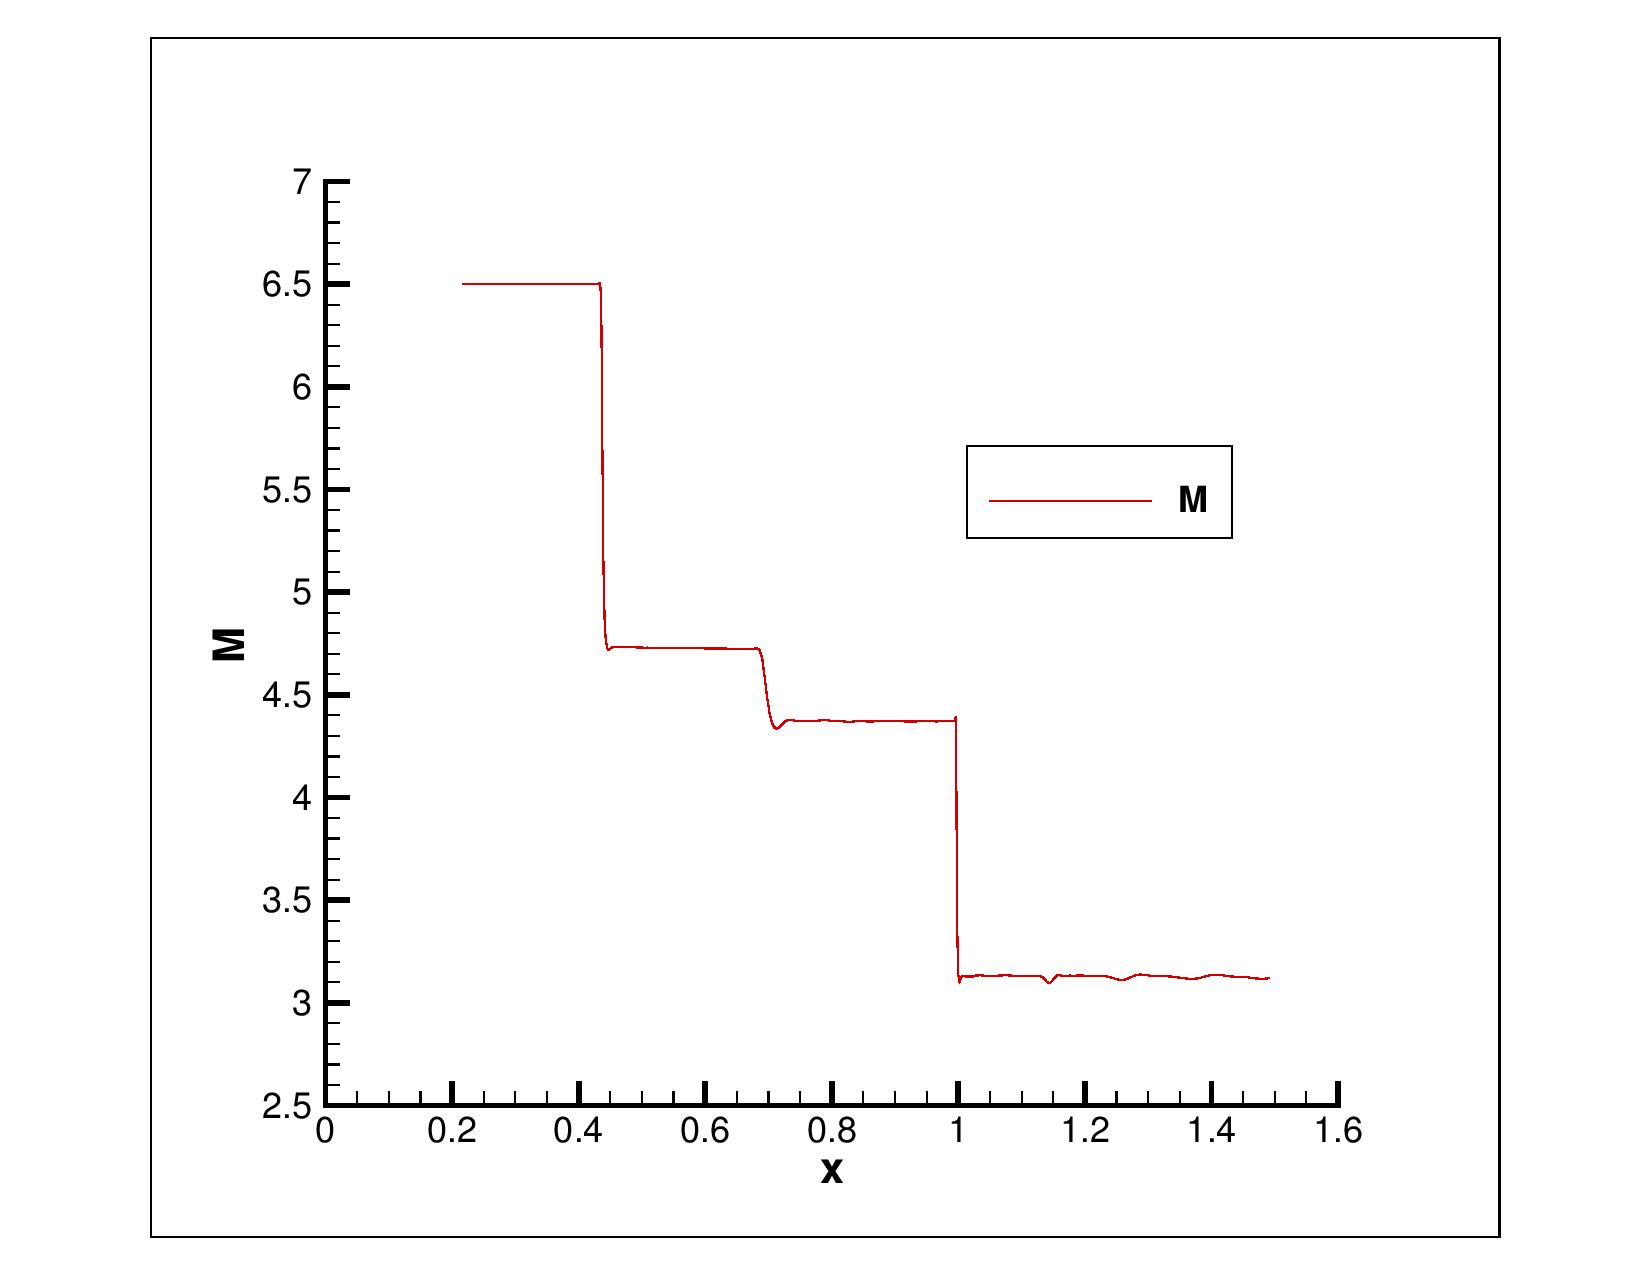
\includegraphics[width=10cm]{6.5/Mach_1.jpg}		%%%%%%%%%%%change location and name
\label{figure:}
\caption{Mach Number jumps across the shocks.}
\end{figure}

\begin{figure}[H]   \label{figure}
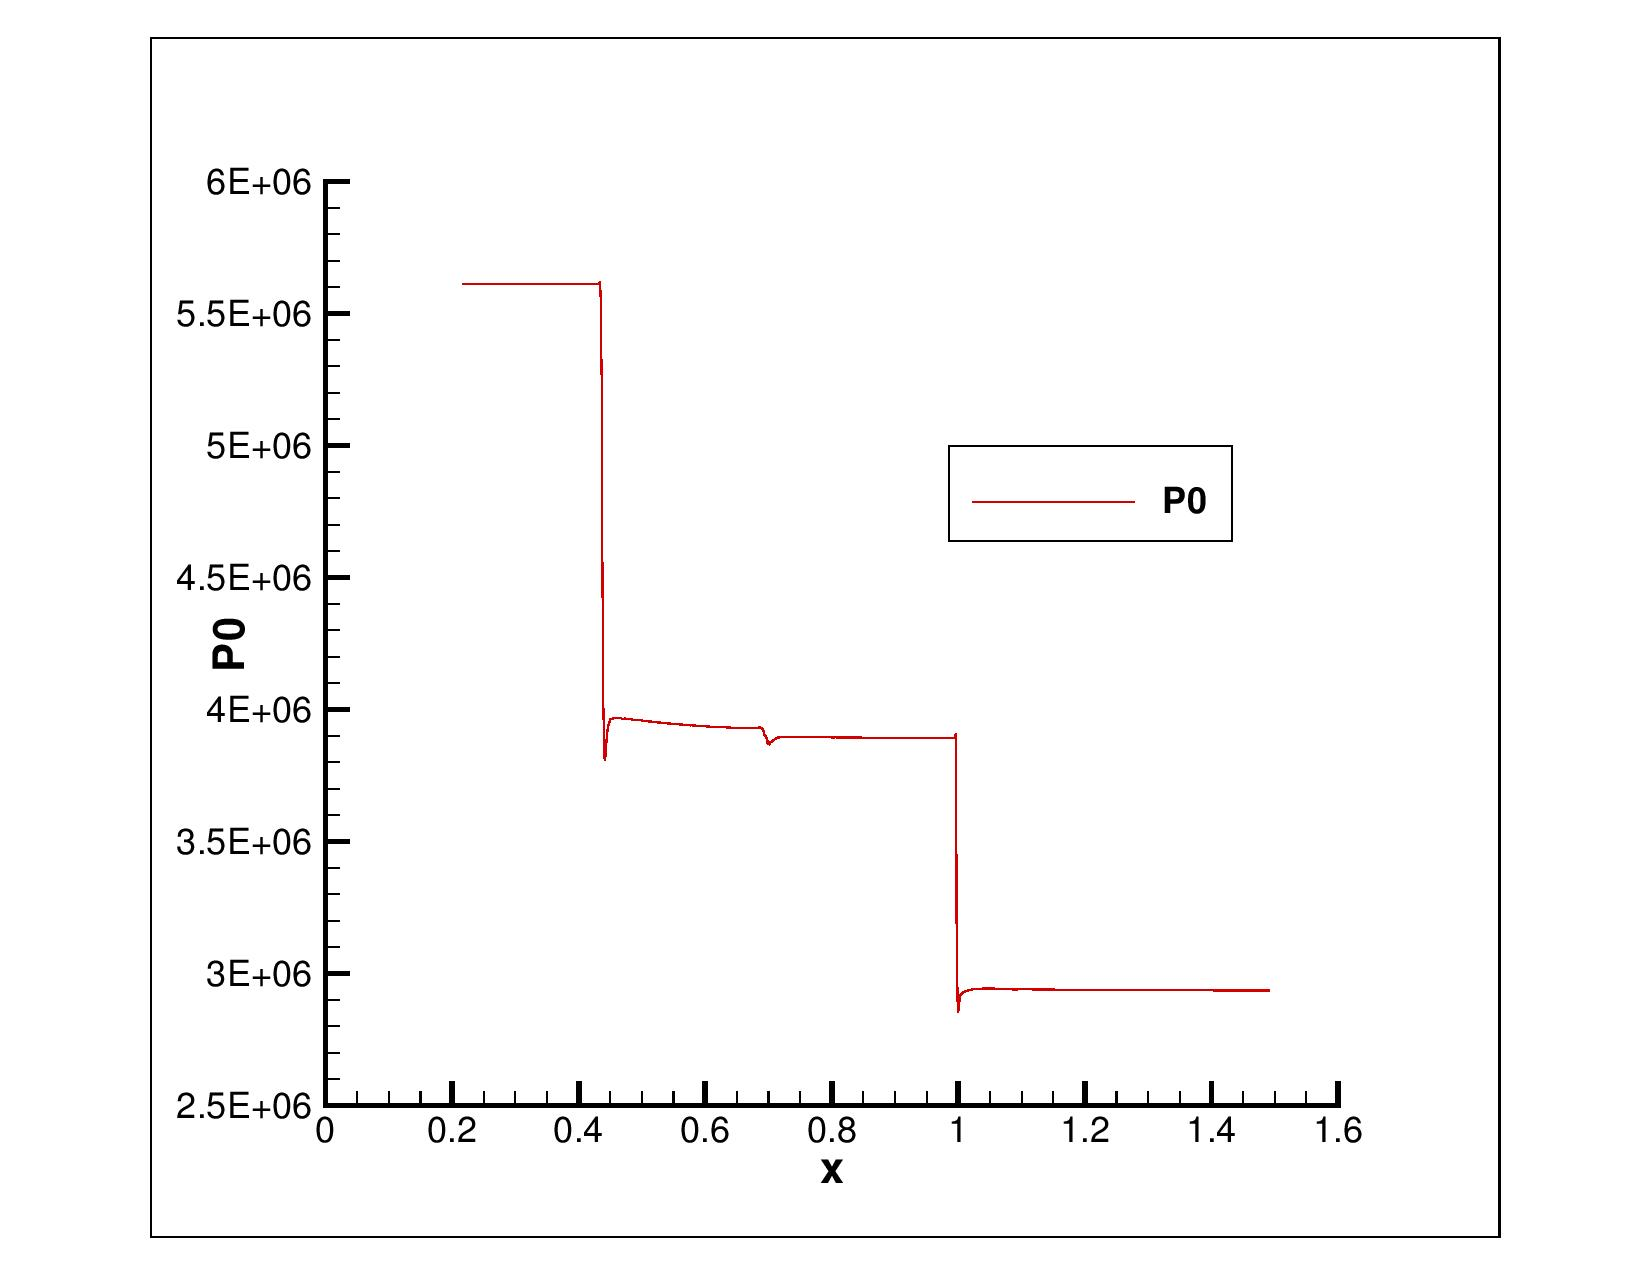
\includegraphics[width=10cm]{6.5/P_total_1.jpg}		%%%%%%%%%%%change location and name
\label{figure:}
\caption{Total Pressure jumps across the shocks.}
\end{figure}

\begin{figure}[H]   \label{figure}
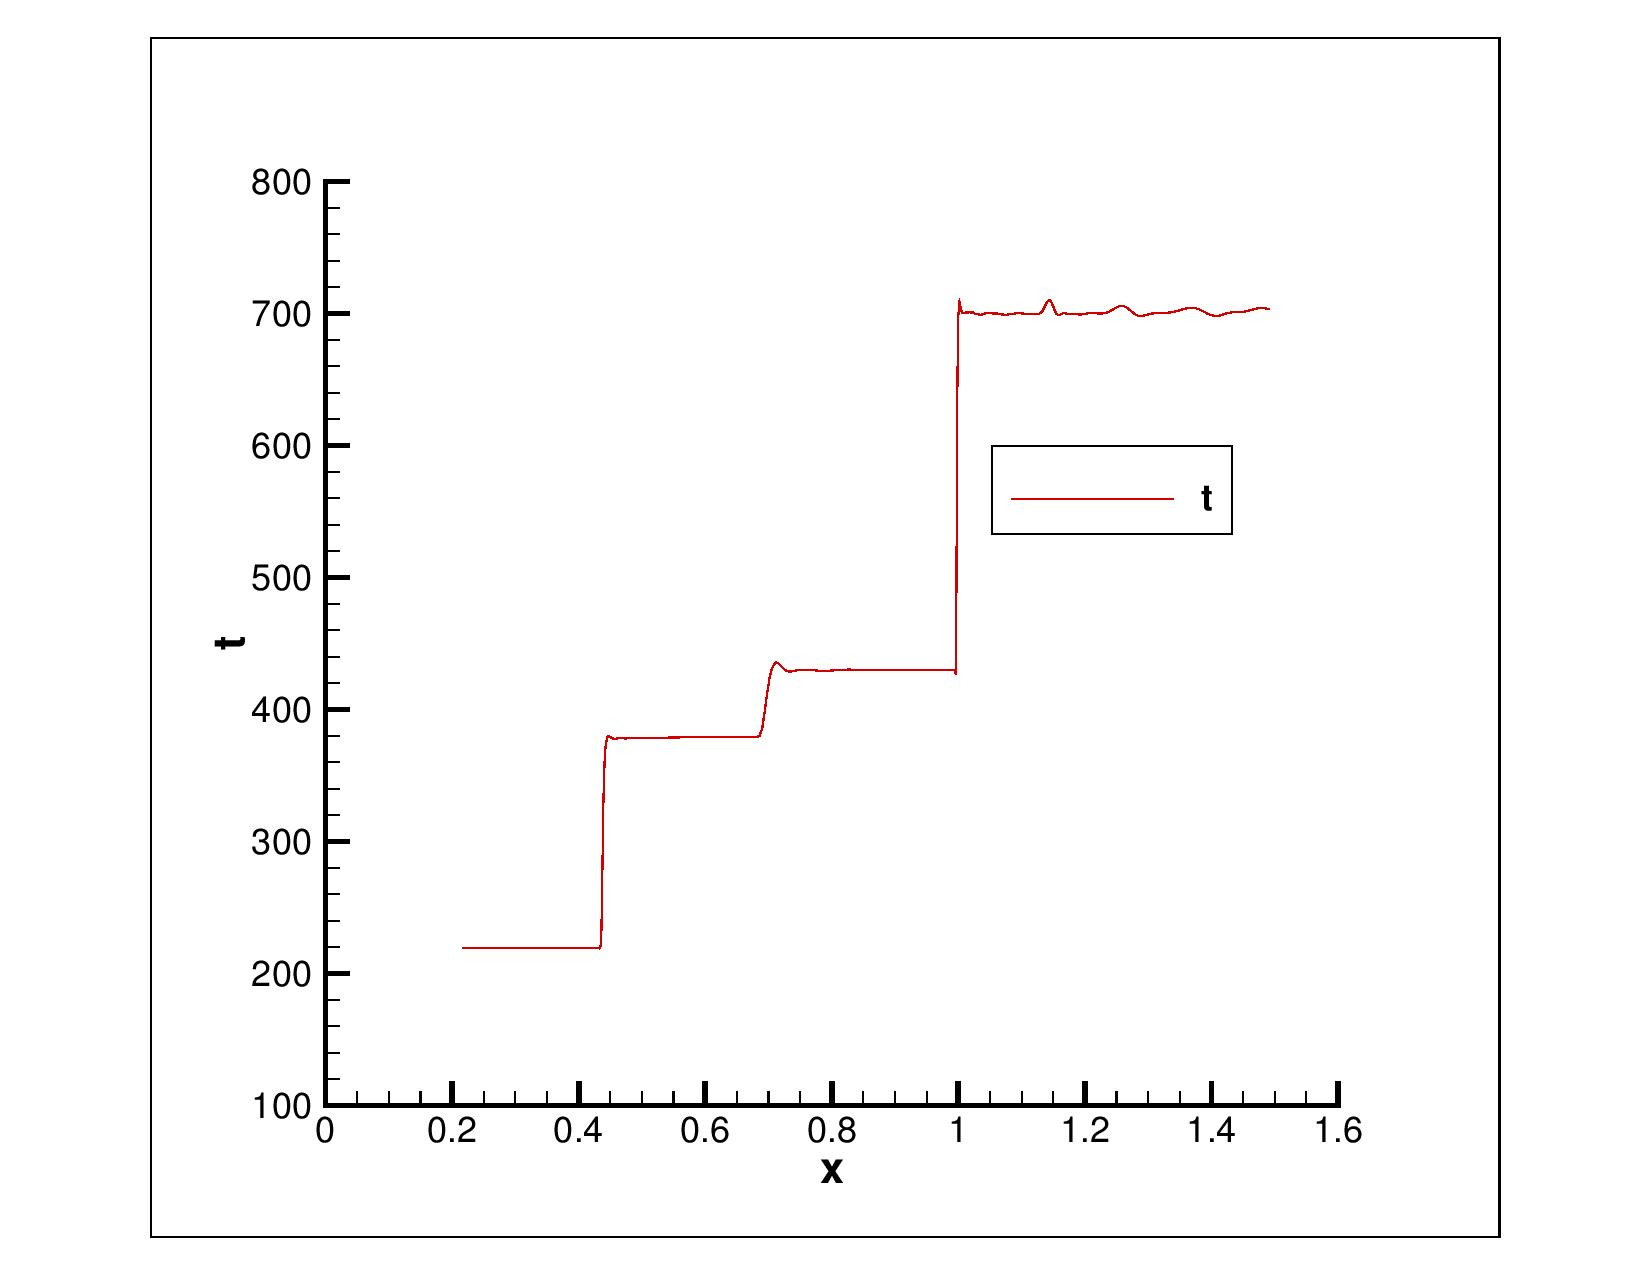
\includegraphics[width=10cm]{6.5/Temp_1.jpg}		%%%%%%%%%%%change location and name
\label{figure:}
\caption{Temperature jumps across the shocks.}
\end{figure}

\newpage
\subsection*{M = 5.5, aoa = $-3^o$}
\begin{figure}[H]   \label{figure}
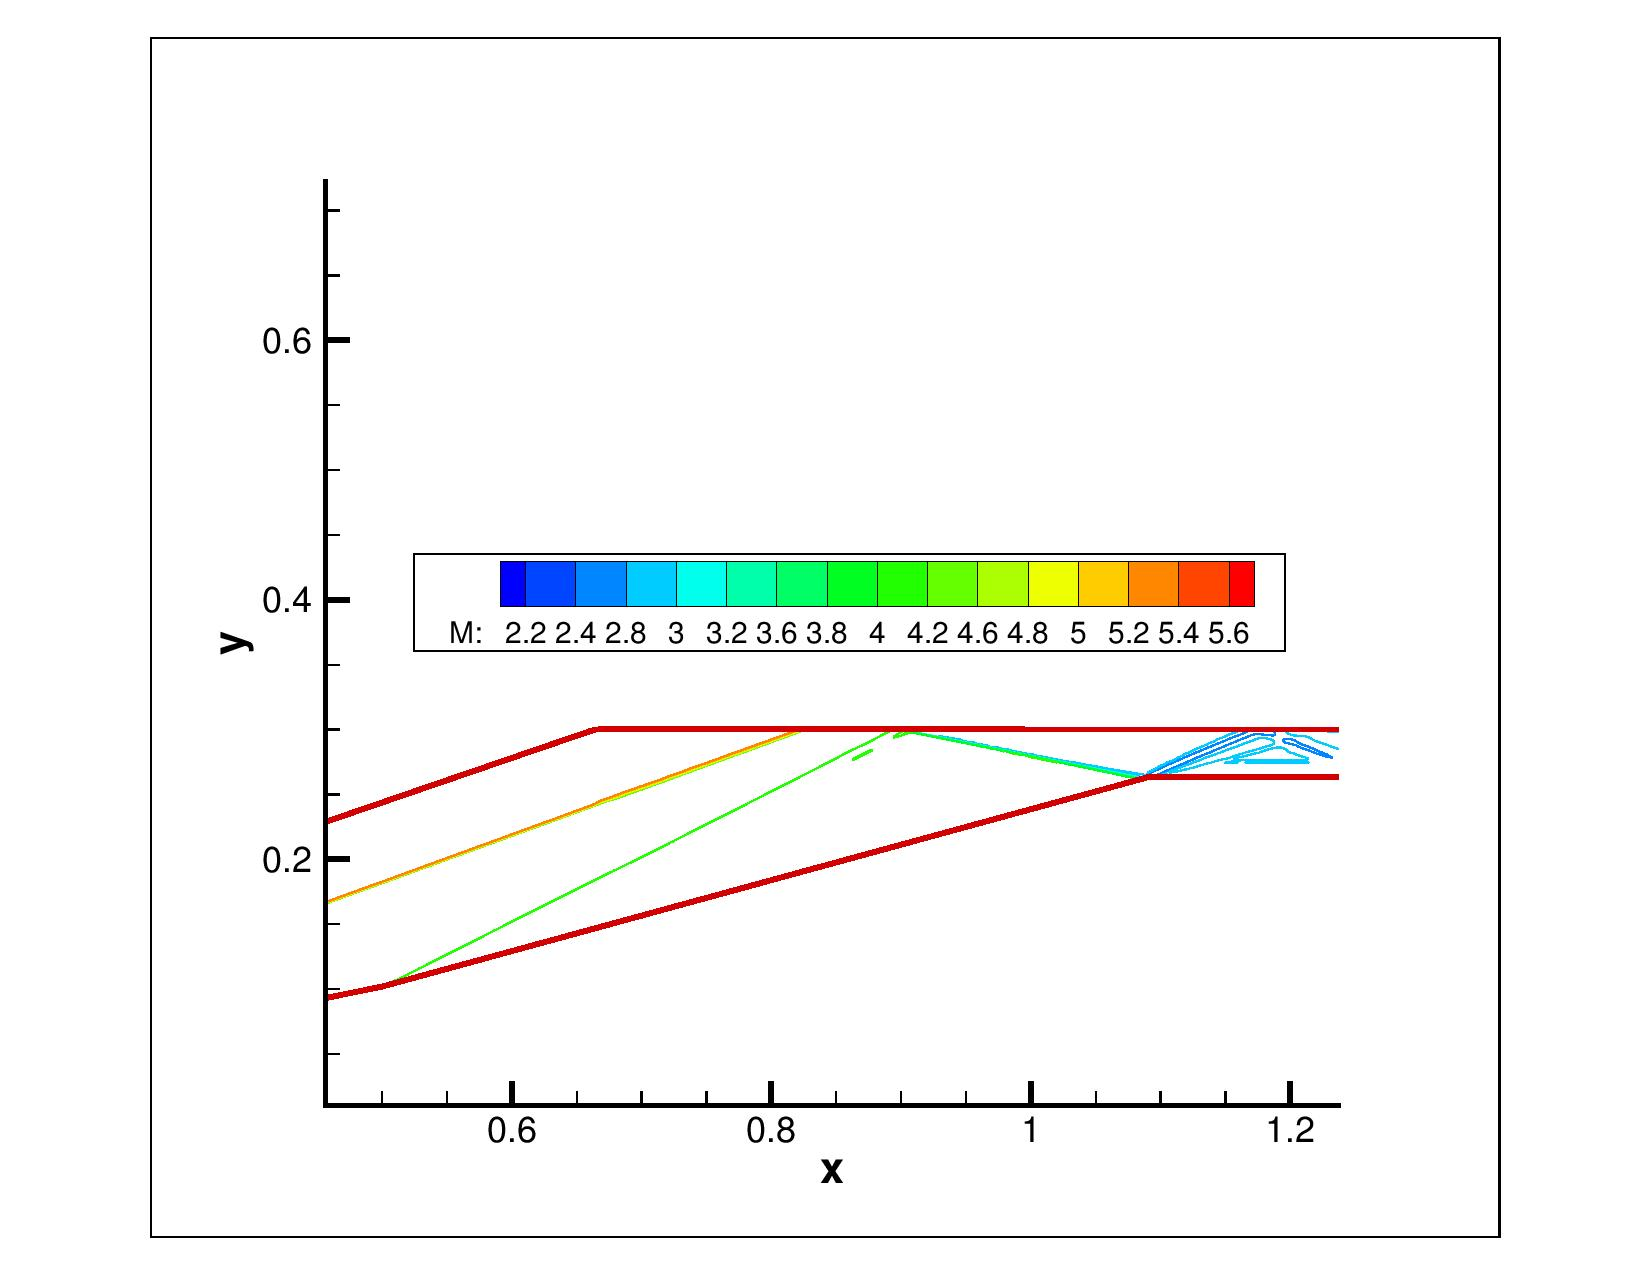
\includegraphics[width=10cm]{5.5/M_cont_2.jpg}		%%%%%%%%%%%change location and name
\label{figure:}
\caption{Mach number Contour Plot}
\end{figure}

\begin{figure}[H]   \label{figure}
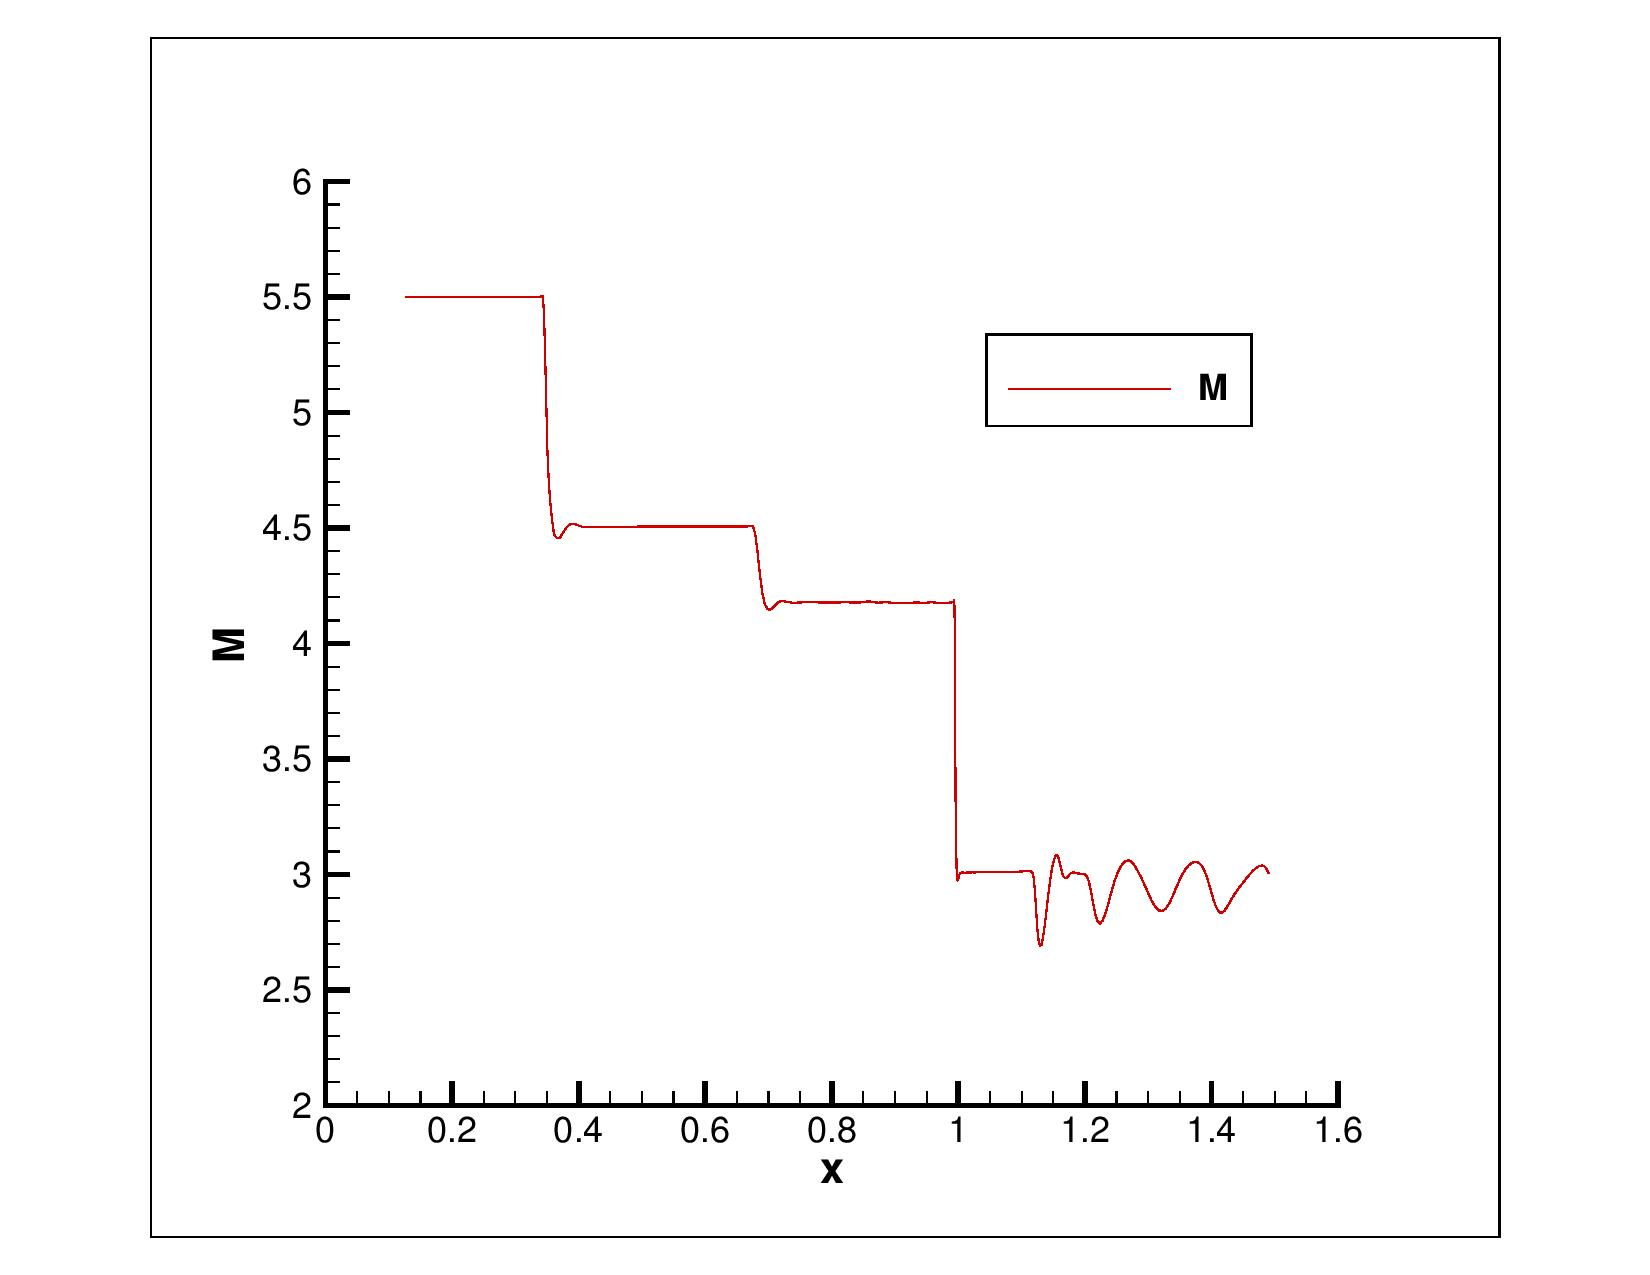
\includegraphics[width=10cm]{5.5/Mach_2.jpg}		%%%%%%%%%%%change location and name
\label{figure:}
\caption{Mach Number jumps across the shocks.}
\end{figure}

\begin{figure}[H]   \label{figure}
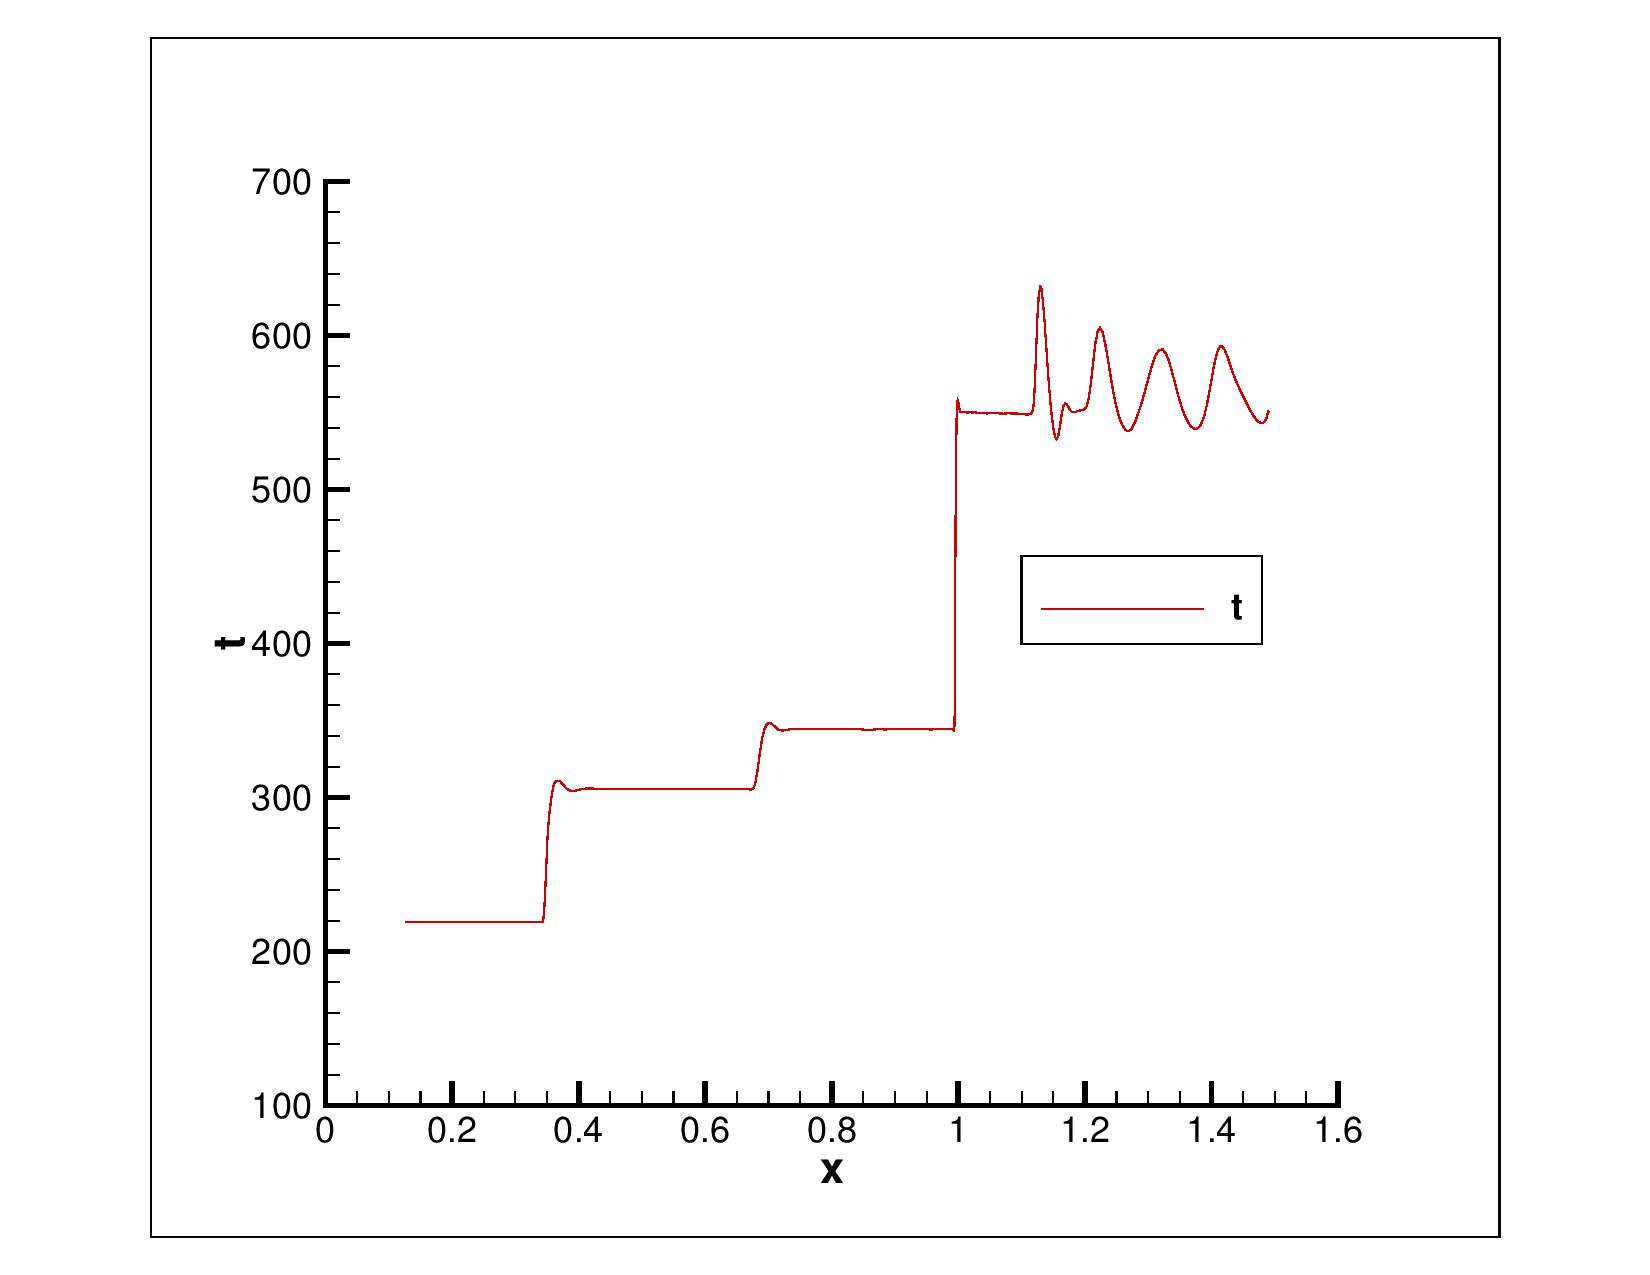
\includegraphics[width=10cm]{5.5/Temp_2.jpg}		%%%%%%%%%%%change location and name
\label{figure:}
\caption{Temperature jumps across the shocks.}
\end{figure}

\begin{figure}[H]   \label{figure}
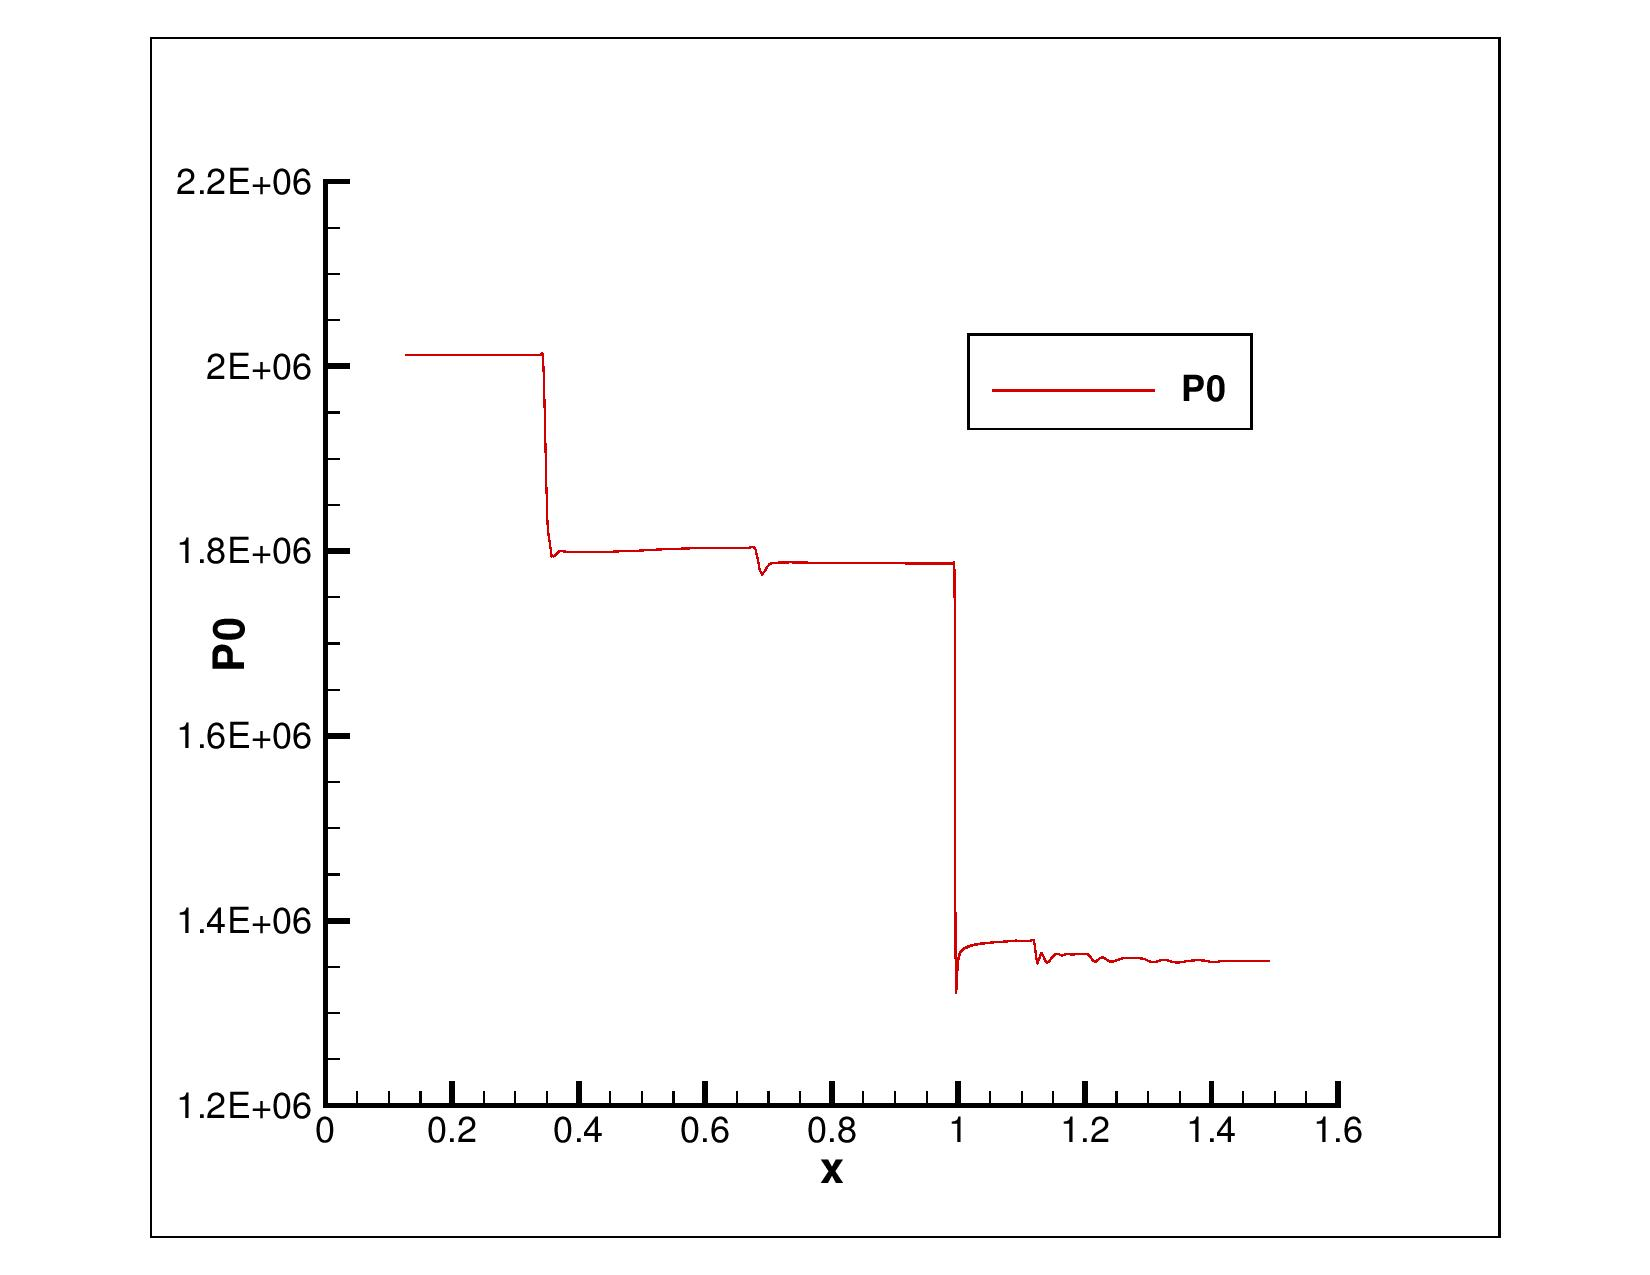
\includegraphics[width=10cm]{5.5/P_total_2.jpg}		%%%%%%%%%%%change location and name
\label{figure:}
\caption{Total Pressure jumps across the shocks.}
\end{figure}

\begin{figure}[H]   \label{figure}
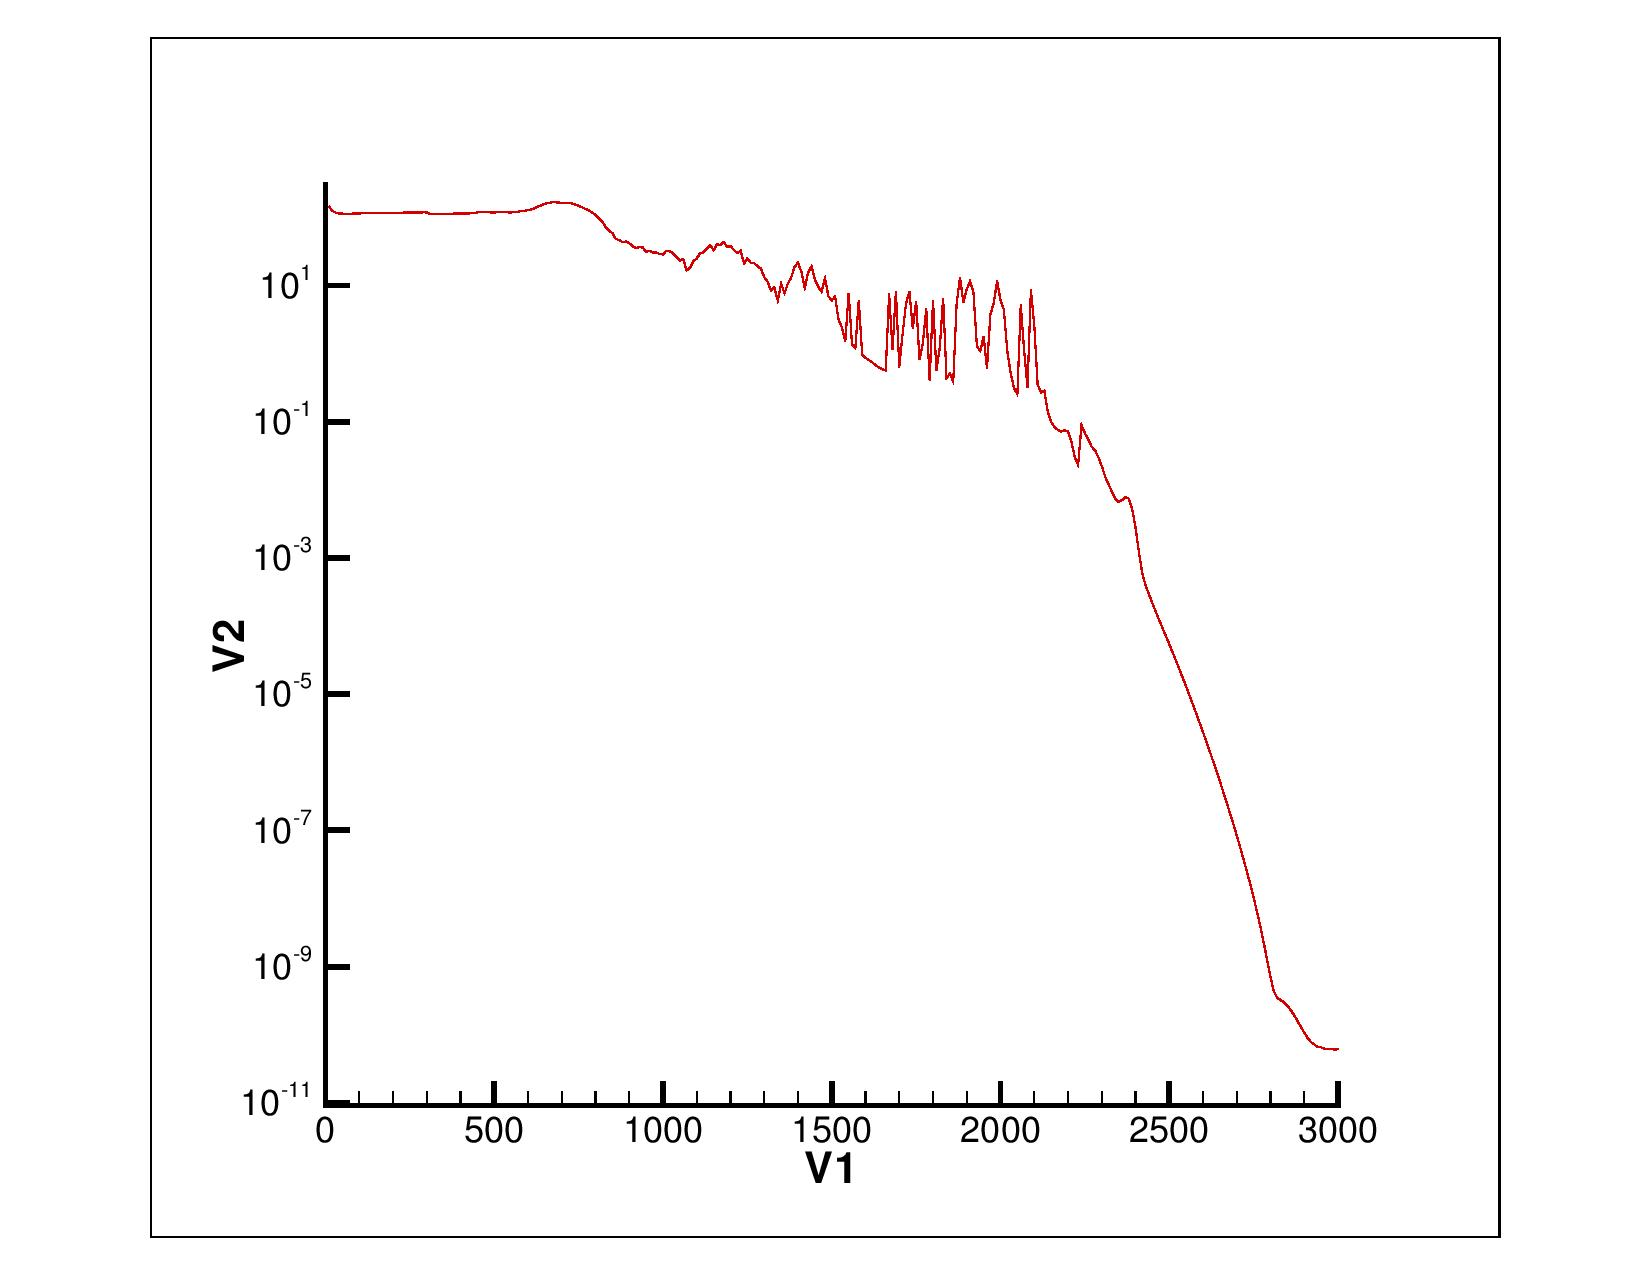
\includegraphics[width=10cm]{5.5/resid_2.jpg}		%%%%%%%%%%%change location and name
\label{figure:}
\caption{Residue Plot for convergence.}
\end{figure}

\newpage
\section*{Comparison of Numerical Results with Inviscid Theory Results}
\subsection*{M = 6.5, aoa = 0}
$\theta1 = 15.292, \theta2 = 11.518$
\begin{table}[h]
  \centering
  \caption{}
  \label{tab:table2}
  \begin{tabular}{l||c|r}
    Flow Properties & Numerical & Theoretical\\
    \hline
    $M1$ & 6.5 & 6.5\\
    \hline
    $M2$ & 4.718 & 4.7185\\
    \hline
    $M3$ & 4.366 & 4.3668\\
    \hline
    $M4$ & 3.120 & 3.1271\\
    \hline
    $P_{o2}/P_{o1}$ & 0.7082 & 0.69498\\
    \hline
    $P_{o3}/P_{o2}$ & 0.9971 & 0.9920\\
    \hline
    $P_{o4}/P_{o3}$ & 0.7720 & 0.75516\\
    \hline
    $T_{4}/T_{1}$ & 3.182 & 3.21\\
    \hline
    Total Pressure loss & 47.65  & 47.938\\
    
  \end{tabular}
\end{table}

\subsection*{M = 5.5, aoa = $-3^o$}
$\theta1 = 12.292, \theta2 = 8.518$
\begin{table}[h]
  \centering
  \caption{}
  \label{tab:table1}
  \begin{tabular}{l||c|r}
    Flow Properties & Numerical & Theoretical\\
    \hline
    $M1$ & 5.5 & 5.5\\
    \hline
    $M2$ & 4.508 & 4.5028\\
    \hline
    $M3$ & 4.177& 4.2753\\
    \hline
    $M4$ & 3.0112 & 3.242\\
    \hline
    $P_{o2}/P_{o1}$ & 0.8950 & 0.8916\\
    \hline
    $P_{o3}/P_{o2}$ & 0.9532 & 0.9920\\
    \hline
    $P_{o4}/P_{o3}$ & 0.8628 & 0.0.7611\\
    \hline
    $T_{4}/T_{1}$ & 2.506 & 2.2222\\
    \hline
    Total Pressure loss & $32.6\%$ & $23.61\%$\\
    
  \end{tabular}
\end{table}

\newpage
\section*{Observations}
Different domain sizes and grid sizes were tried and the following observations were made -
\begin{enumerate}
\item It can be seen from the plots above, that the flow is decelerated and compressed in the inlet region, thus, mach number decreases, temperature increases, total pressure decreases ( converted in the form of heat) and density increases.
\item From the mach number contour plot, it is clear that two shock wave emerging from the two ramps do not intersect on the cowl. This happens when free stream mach number is less than design mach number. (design mach number in this case is 6.5).
\item From figure 9, it can be seen that residue is high till 2200 iterations after which there is a steep decrease in residue to around $10^{-9}$ after 3000 iterations.
\item Static temperature gain is lower in case of Mach number 5.5, $aoa = -3^o$ than Mach number 6.5, $aoa = 0^o$ while, overall total pressure loss is greater for the design condition.
\item In case of mach number 5.5, $aoa = -3^o$, the number of mach waves are more than design condition, therefore, compression region of scramjet engine is higher. This also led to fluctuations in pressure and temperature plots as can be seen in figure 6 and 7.
\item Such fluctutations (or mach waves) do not occur in design condition because the reflected shock from the cowl tip exactly cancels these mach waves.
\item Numerical results for our case maches closely with the inviscid theory results, except in region 4, where the difference in mach number, pressure, and temperature is higher than rest of the regions. This happened because we didn't take into account the mach waves that will emerge after the 3rd shock while using inviscid theory.
\end{enumerate}

\end{document}
